\begin{figure*}[p]
  \centering
    \captionsetup[subfigure]{font=tiny, skip=0pt}
  
  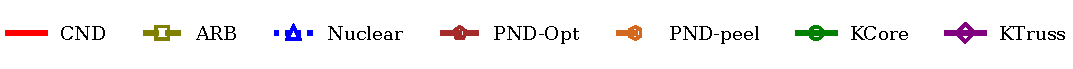
\includegraphics[width=0.9\linewidth]{figure/legend_algorithms_fixed_lines.pdf}

    \begin{minipage}[c]{0.02\textwidth}
    \centering
    \raisebox{2em}{\rotatebox{90}{\tiny \textbf{Time(s)}}} 
  \end{minipage}  \begin{subfigure}[t]{0.158\textwidth}
    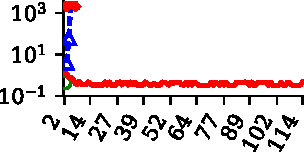
\includegraphics[width=\linewidth]{figure/com-dblp_r1_time_by_s_No_Hi.pdf}
    \caption{\myaddRA{dblp $s\{r{=}1\}$}}
  \end{subfigure}\hfill
  \begin{subfigure}[t]{0.158\textwidth}
    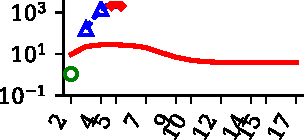
\includegraphics[width=\linewidth]{figure/com-youtube_r1_time_by_s_No_Hi.pdf}
    \caption{YT $s\{r{=}1\}$}
  \end{subfigure}\hfill
  \begin{subfigure}[t]{0.158\textwidth}
    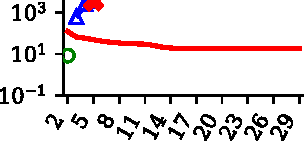
\includegraphics[width=\linewidth]{figure/soc-pokec-relationships_r1_time_by_s_No_Hi.pdf}
    \caption{pokec $s\{r{=}1\}$}
  \end{subfigure}\hfill
  \begin{subfigure}[t]{0.158\textwidth}
    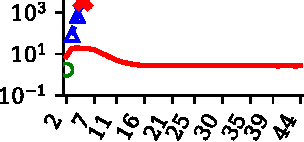
\includegraphics[width=\linewidth]{figure/web-Google_r1_time_by_s_No_Hi.pdf}
    \caption{Google $s\{r{=}1\}$}
  \end{subfigure}\hfill
  \begin{subfigure}[t]{0.158\textwidth}
    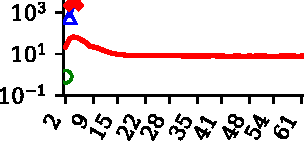
\includegraphics[width=\linewidth]{figure/web-Stanford_r1_time_by_s_No_Hi.pdf}
    \caption{Stanford $s\{r{=}1\}$}
  \end{subfigure}\hfill
  \begin{subfigure}[t]{0.158\textwidth}
    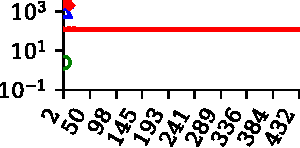
\includegraphics[width=\linewidth]{figure/web-it-2004_r1_time_by_s_No_Hi.pdf}
    \caption{web-it $s\{r{=}1\}$}
  \end{subfigure}
  
  

    \begin{minipage}[c]{0.02\textwidth}
    \centering
    \raisebox{2em}{\rotatebox{90}{\tiny \textbf{Time(s)}}} 
  \end{minipage}  \begin{subfigure}[t]{0.158\textwidth}
    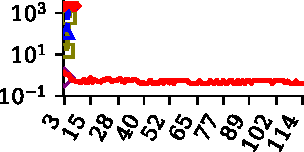
\includegraphics[width=\linewidth]{figure/com-dblp_r2_time_by_s_No_Hi.pdf}
    \caption{\myaddRA{dblp $s\{r{=}2\}$}}
  \end{subfigure}\hfill
  \begin{subfigure}[t]{0.158\textwidth}
    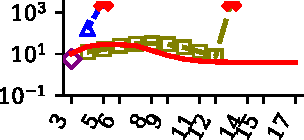
\includegraphics[width=\linewidth]{figure/com-youtube_r2_time_by_s_No_Hi.pdf}
    \caption{YT $s\{r{=}2\}$}
    \label{fig:youtube_r2_time_by_s}
  \end{subfigure}\hfill
  \begin{subfigure}[t]{0.158\textwidth}
    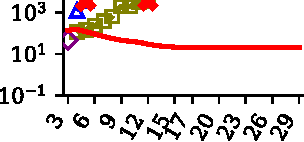
\includegraphics[width=\linewidth]{figure/soc-pokec-relationships_r2_time_by_s_No_Hi.pdf}
    \caption{pokec $s\{r{=}2\}$}
  \end{subfigure}\hfill
  \begin{subfigure}[t]{0.158\textwidth}
    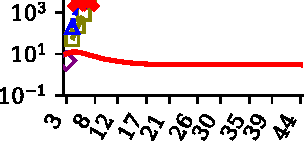
\includegraphics[width=\linewidth]{figure/web-Google_r2_time_by_s_No_Hi.pdf}
    \caption{Google $s\{r{=}2\}$}
  \end{subfigure}\hfill
  \begin{subfigure}[t]{0.158\textwidth}
    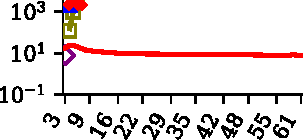
\includegraphics[width=\linewidth]{figure/web-Stanford_r2_time_by_s_No_Hi.pdf}
    \caption{Stanford $s\{r{=}2\}$}
  \end{subfigure}\hfill
  \begin{subfigure}[t]{0.158\textwidth}
    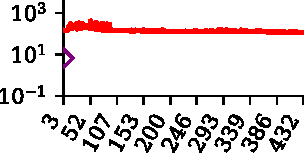
\includegraphics[width=\linewidth]{figure/web-it-2004_r2_time_by_s_No_Hi.pdf}
    \caption{web-it $s\{r{=}2\}$}
  \end{subfigure}

  
  \caption{Running time (seconds) across $s$ without hierarchy for $r = 1$(a-f) and $r=2$(g-l).}
  \label{fig:r1r2_time_by_s}

  
    \begin{minipage}[c]{0.02\textwidth}
    \centering
    \raisebox{2em}{\rotatebox{90}{\tiny \textbf{Time(s)}}} 
  \end{minipage}  \begin{subfigure}[t]{0.158\textwidth}
    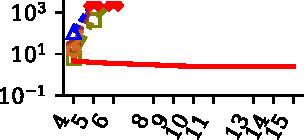
\includegraphics[width=\linewidth]{figure/com-dblp_r3_time_by_s_No_Hi.pdf}
    \caption{\myaddRA{dblp $s\{r{=}3\}$}}
  \end{subfigure}\hfill
  \begin{subfigure}[t]{0.158\textwidth}
    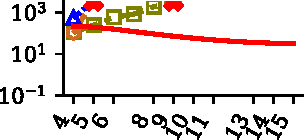
\includegraphics[width=\linewidth]{figure/soc-pokec-relationships_r3_time_by_s_No_Hi.pdf}
    \caption{pokec $s\{r{=}3\}$}
  \end{subfigure}\hfill
  \begin{subfigure}[t]{0.158\textwidth}
    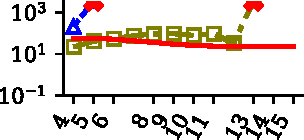
\includegraphics[width=\linewidth]{figure/com-youtube_r3_time_by_s_No_Hi.pdf}
    \caption{YT $s\{r{=}3\}$}
  \end{subfigure}\hfill
  \begin{subfigure}[t]{0.158\textwidth}
    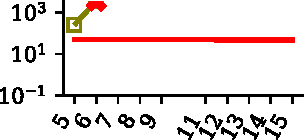
\includegraphics[width=\linewidth]{figure/com-dblp_r4_time_by_s_No_Hi.pdf}
    \caption{dblp $s\{r{=}4\}$}
  \end{subfigure}\hfill
  \begin{subfigure}[t]{0.158\textwidth}
    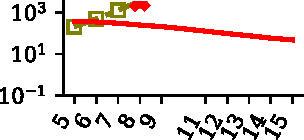
\includegraphics[width=\linewidth]{figure/soc-pokec-relationships_r4_time_by_s_No_Hi.pdf}
    \caption{pokec $s\{r{=}4\}$}
  \end{subfigure}\hfill
  \begin{subfigure}[t]{0.158\textwidth}
    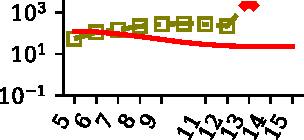
\includegraphics[width=\linewidth]{figure/com-youtube_r4_time_by_s_No_Hi.pdf}
    \caption{YT $s\{r{=}4\}$}
  \end{subfigure}

  

    \begin{minipage}[c]{0.02\textwidth}
    \centering
    \raisebox{2em}{\rotatebox{90}{\tiny \textbf{Time(s)}}} 
  \end{minipage}  \begin{subfigure}[t]{0.158\textwidth}
    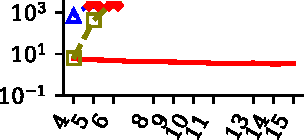
\includegraphics[width=\linewidth]{figure/com-dblp_r3_time_by_s.pdf}
    \caption{dblp $s\{r{=}3\}$}
  \end{subfigure}\hfill
  \begin{subfigure}[t]{0.158\textwidth}
    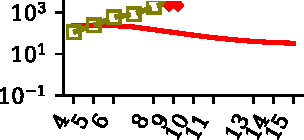
\includegraphics[width=\linewidth]{figure/soc-pokec-relationships_r3_time_by_s.pdf}
    \caption{pokec $s\{r{=}3\}$}
  \end{subfigure}\hfill
  \begin{subfigure}[t]{0.158\textwidth}
    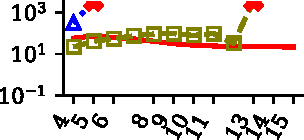
\includegraphics[width=\linewidth]{figure/com-youtube_r3_time_by_s.pdf}
    \caption{YT $s\{r{=}3\}$}
  \end{subfigure}\hfill
  \begin{subfigure}[t]{0.158\textwidth}
    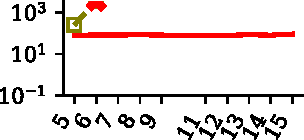
\includegraphics[width=\linewidth]{figure/com-dblp_r4_time_by_s.pdf}
    \caption{dblp $s\{r{=}4\}$}
  \end{subfigure}\hfill
  \begin{subfigure}[t]{0.158\textwidth}
    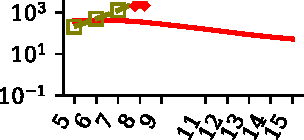
\includegraphics[width=\linewidth]{figure/soc-pokec-relationships_r4_time_by_s.pdf}
    \caption{pokec $s\{r{=}4\}$}
  \end{subfigure}\hfill
  \begin{subfigure}[t]{0.158\textwidth}
    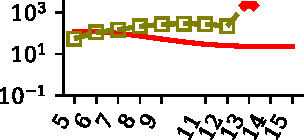
\includegraphics[width=\linewidth]{figure/com-youtube_r4_time_by_s.pdf}
    \caption{YT $s\{r{=}4\}$}
  \end{subfigure}

  
  \caption{Running time (seconds) across $s$ for $r \in \{3,4\}$(a-f without hierarchy; g-l with hierarchy).}
  \label{fig:time_by_s_r3_r4_combined}

  
    \begin{minipage}[c]{0.02\textwidth}
    \centering
    \raisebox{2em}{\rotatebox{90}{\tiny \textbf{Time(s)}}} 
  \end{minipage}  \begin{subfigure}[t]{0.158\textwidth}
      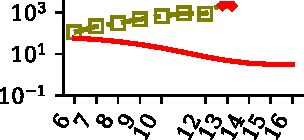
\includegraphics[width=\linewidth]{figure/com-youtube_r5_time_by_s_No_Hi.pdf}
      \caption{YT $s\{r{=}5\}$}
  \end{subfigure}\hfill
  \begin{subfigure}[t]{0.158\textwidth}
      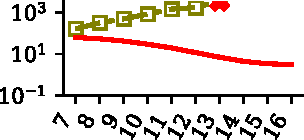
\includegraphics[width=\linewidth]{figure/com-youtube_r6_time_by_s_No_Hi.pdf}
      \caption{YT $s\{r{=}6\}$}
  \end{subfigure}\hfill
  \begin{subfigure}[t]{0.158\textwidth}
      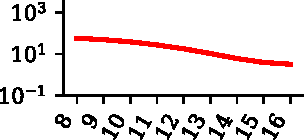
\includegraphics[width=\linewidth]{figure/com-youtube_r7_time_by_s_No_Hi.pdf}
      \caption{YT $s\{r{=}7\}$}
  \end{subfigure}\hfill
  \begin{subfigure}[t]{0.158\textwidth}
      \includegraphics[width=\linewidth]{figure/soc-pokec-relationships_r5_time_by_s_no_hi.eps}
      \caption{pokec $s\{r{=}5\}$}
  \end{subfigure}\hfill
  \begin{subfigure}[t]{0.158\textwidth}
      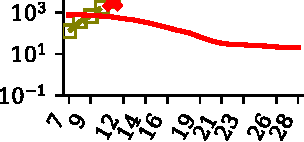
\includegraphics[width=\linewidth]{figure/soc-pokec-relationships_r6_time_by_s_no_hi.pdf}
      \caption{pokec $s\{r{=}6\}$}
  \end{subfigure}\hfill
  \begin{subfigure}[t]{0.158\textwidth}
      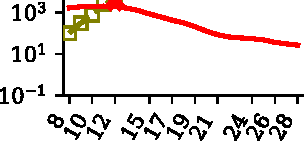
\includegraphics[width=\linewidth]{figure/soc-pokec-relationships_r7_time_by_s_no_hi.pdf}
      \caption{pokec $s\{r{=}7\}$}
  \end{subfigure}

  
  \caption{Running time (seconds) across $s$ without hierarchy for $r \in \{5,6,7\}$.}
  \label{fig:time_by_s_r5_r7_combined}

  
    

    \begin{minipage}[c]{0.02\textwidth}
    \centering
    \raisebox{3em}{\rotatebox{90}{\tiny \textbf{Mem(MB)}}} 
  \end{minipage}  \begin{subfigure}[t]{0.158\textwidth}
    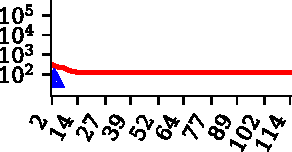
\includegraphics[width=\linewidth]{figure/com-dblp_r1_memory_by_s_no_hi.pdf}
    \caption{dblp $s\{r{=}1\}$}
  \end{subfigure}\hfill
  \begin{subfigure}[t]{0.158\textwidth}
    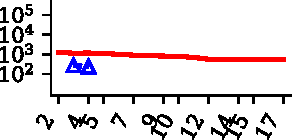
\includegraphics[width=\linewidth]{figure/com-youtube_r1_memory_by_s_no_hi.pdf}
    \caption{YT $s\{r{=}1\}$}
  \end{subfigure}\hfill
  \begin{subfigure}[t]{0.158\textwidth}
    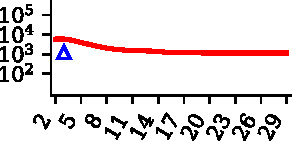
\includegraphics[width=\linewidth]{figure/soc-pokec-relationships_r1_memory_by_s_no_hi.pdf}
    \caption{pokec $s\{r{=}1\}$}
  \end{subfigure}\hfill
  \begin{subfigure}[t]{0.158\textwidth}
    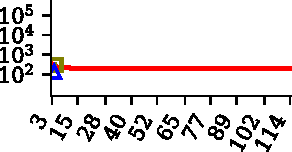
\includegraphics[width=\linewidth]{figure/com-dblp_r2_memory_by_s_no_hi.pdf}
    \caption{dblp $s\{r{=}2\}$}
  \end{subfigure}\hfill
  \begin{subfigure}[t]{0.158\textwidth}
    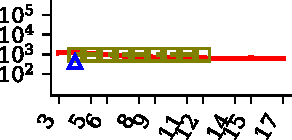
\includegraphics[width=\linewidth]{figure/com-youtube_r2_memory_by_s_no_hi.pdf}
    \caption{YT $s\{r{=}2\}$}
  \end{subfigure}\hfill
  \begin{subfigure}[t]{0.158\textwidth}
    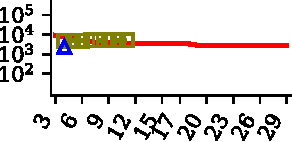
\includegraphics[width=\linewidth]{figure/soc-pokec-relationships_r2_memory_by_s_no_hi.pdf}
    \caption{pokec $s\{r{=}2\}$}
  \end{subfigure}

  

    \begin{minipage}[c]{0.02\textwidth}
    \centering
    \raisebox{3em}{\rotatebox{90}{\tiny \textbf{Mem(MB)}}}
  \end{minipage}  \begin{subfigure}[t]{0.158\textwidth}
    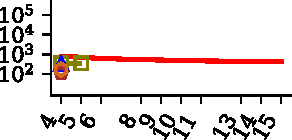
\includegraphics[width=\linewidth]{figure/com-dblp_r3_memory_by_s_no_hi.pdf}
    \caption{dblp $s\{r{=}3\}$}
  \end{subfigure}\hfill
  \begin{subfigure}[t]{0.158\textwidth}
    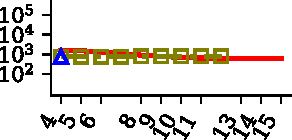
\includegraphics[width=\linewidth]{figure/com-youtube_r3_memory_by_s_no_hi.pdf}
    \caption{YT $s\{r{=}3\}$}
  \end{subfigure}\hfill
  \begin{subfigure}[t]{0.158\textwidth}
    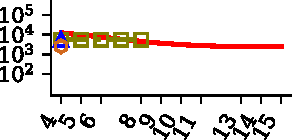
\includegraphics[width=\linewidth]{figure/soc-pokec-relationships_r3_memory_by_s_no_hi.pdf}
    \caption{pokec $s\{r{=}3\}$}
  \end{subfigure}\hfill
  \begin{subfigure}[t]{0.158\textwidth}
    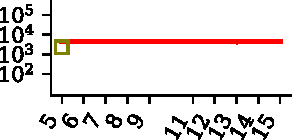
\includegraphics[width=\linewidth]{figure/com-dblp_r4_memory_by_s_no_hi.pdf}
    \caption{dblp $s\{r{=}4\}$}
  \end{subfigure}\hfill
  \begin{subfigure}[t]{0.158\textwidth}
    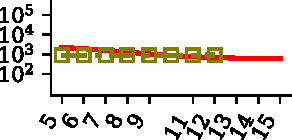
\includegraphics[width=\linewidth]{figure/com-youtube_r4_memory_by_s_no_hi.pdf}
    \caption{YT $s\{r{=}4\}$}
  \end{subfigure}\hfill
  \begin{subfigure}[t]{0.158\textwidth}
    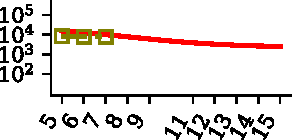
\includegraphics[width=\linewidth]{figure/soc-pokec-relationships_r4_memory_by_s_no_hi.pdf}
    \caption{pokec $s\{r{=}4\}$}
  \end{subfigure}

  
  \caption{Time and Memory usage comparison for ($r \in \{1,2,3,4\}$).}
  \label{fig:mem_panel_b}

\end{figure*}
